% This file is generated by the MATLAB m-file laprint.m. It can be included
% into LaTeX documents using the packages graphicx, color and psfrag.
% It is accompanied by a postscript file. A sample LaTeX file is:
%    \documentclass{article}\usepackage{graphicx,color,psfrag}
%    \begin{document}% This file is generated by the MATLAB m-file laprint.m. It can be included
% into LaTeX documents using the packages graphicx, color and psfrag.
% It is accompanied by a postscript file. A sample LaTeX file is:
%    \documentclass{article}\usepackage{graphicx,color,psfrag}
%    \begin{document}% This file is generated by the MATLAB m-file laprint.m. It can be included
% into LaTeX documents using the packages graphicx, color and psfrag.
% It is accompanied by a postscript file. A sample LaTeX file is:
%    \documentclass{article}\usepackage{graphicx,color,psfrag}
%    \begin{document}% This file is generated by the MATLAB m-file laprint.m. It can be included
% into LaTeX documents using the packages graphicx, color and psfrag.
% It is accompanied by a postscript file. A sample LaTeX file is:
%    \documentclass{article}\usepackage{graphicx,color,psfrag}
%    \begin{document}\input{meas}\end{document}
% See http://www.mathworks.de/matlabcentral/fileexchange/loadFile.do?objectId=4638
% for recent versions of laprint.m.
%
% created by:           LaPrint version 3.16 (13.9.2004)
% created on:           01-Apr-2014 19:01:39
% eps bounding box:     15 cm x 11.0893 cm
% comment:              
%
%\begin{psfrags}%
%\psfragscanon%
%
% text strings:
\psfrag{s03}[t][t]{\color[rgb]{0,0,0}\setlength{\tabcolsep}{0pt}\begin{tabular}{c}Time [hours]\end{tabular}}%
\psfrag{s04}[b][b]{\color[rgb]{0,0,0}\setlength{\tabcolsep}{0pt}\begin{tabular}{c}$V_\text{cell}$\ $[\text{V}]$\end{tabular}}%
%
% xticklabels:
\psfrag{x01}[t][t]{0}%
\psfrag{x02}[t][t]{5}%
\psfrag{x03}[t][t]{10}%
\psfrag{x04}[t][t]{15}%
\psfrag{x05}[t][t]{20}%
\psfrag{x06}[t][t]{25}%
\psfrag{x07}[t][t]{30}%
%
% yticklabels:
\psfrag{v01}[r][r]{1.5}%
\psfrag{v02}[r][r]{2}%
\psfrag{v03}[r][r]{2.5}%
\psfrag{v04}[r][r]{3}%
\psfrag{v05}[r][r]{3.5}%
\psfrag{v06}[r][r]{4}%
\psfrag{v07}[r][r]{4.5}%
\psfrag{v08}[r][r]{5}%
%
% Figure:
%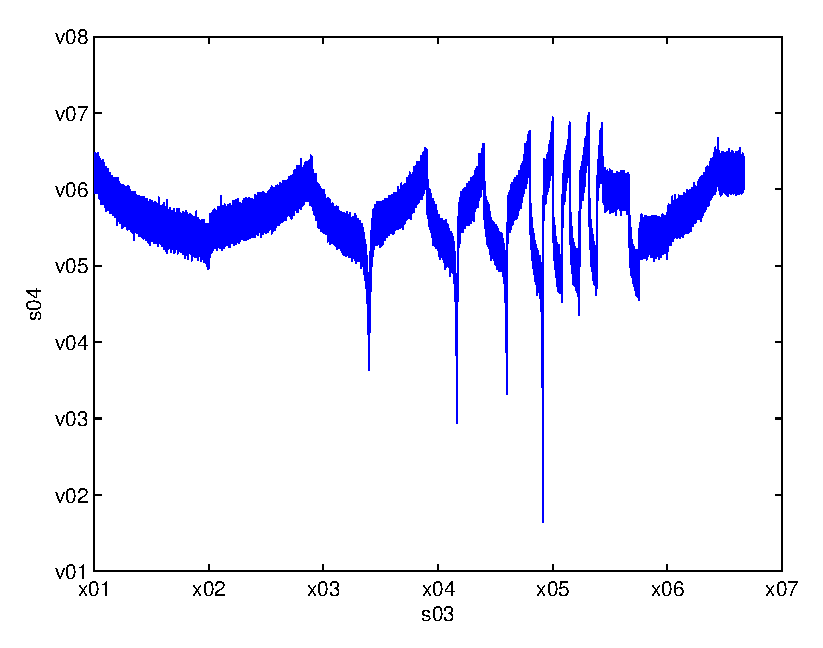
\includegraphics[width=15cm]{meas.eps}%
%\end{psfrags}%
%
% End meas.tex
\end{document}
% See http://www.mathworks.de/matlabcentral/fileexchange/loadFile.do?objectId=4638
% for recent versions of laprint.m.
%
% created by:           LaPrint version 3.16 (13.9.2004)
% created on:           01-Apr-2014 19:01:39
% eps bounding box:     15 cm x 11.0893 cm
% comment:              
%
%\begin{psfrags}%
%\psfragscanon%
%
% text strings:
\psfrag{s03}[t][t]{\color[rgb]{0,0,0}\setlength{\tabcolsep}{0pt}\begin{tabular}{c}Time [hours]\end{tabular}}%
\psfrag{s04}[b][b]{\color[rgb]{0,0,0}\setlength{\tabcolsep}{0pt}\begin{tabular}{c}$V_\text{cell}$\ $[\text{V}]$\end{tabular}}%
%
% xticklabels:
\psfrag{x01}[t][t]{0}%
\psfrag{x02}[t][t]{5}%
\psfrag{x03}[t][t]{10}%
\psfrag{x04}[t][t]{15}%
\psfrag{x05}[t][t]{20}%
\psfrag{x06}[t][t]{25}%
\psfrag{x07}[t][t]{30}%
%
% yticklabels:
\psfrag{v01}[r][r]{1.5}%
\psfrag{v02}[r][r]{2}%
\psfrag{v03}[r][r]{2.5}%
\psfrag{v04}[r][r]{3}%
\psfrag{v05}[r][r]{3.5}%
\psfrag{v06}[r][r]{4}%
\psfrag{v07}[r][r]{4.5}%
\psfrag{v08}[r][r]{5}%
%
% Figure:
%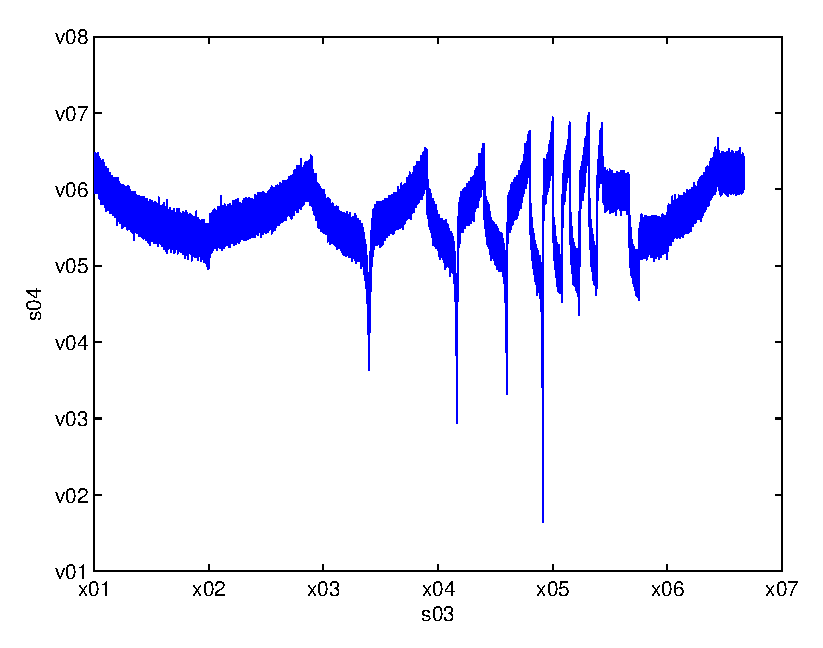
\includegraphics[width=15cm]{meas.eps}%
%\end{psfrags}%
%
% End meas.tex
\end{document}
% See http://www.mathworks.de/matlabcentral/fileexchange/loadFile.do?objectId=4638
% for recent versions of laprint.m.
%
% created by:           LaPrint version 3.16 (13.9.2004)
% created on:           01-Apr-2014 19:01:39
% eps bounding box:     15 cm x 11.0893 cm
% comment:              
%
%\begin{psfrags}%
%\psfragscanon%
%
% text strings:
\psfrag{s03}[t][t]{\color[rgb]{0,0,0}\setlength{\tabcolsep}{0pt}\begin{tabular}{c}Time [hours]\end{tabular}}%
\psfrag{s04}[b][b]{\color[rgb]{0,0,0}\setlength{\tabcolsep}{0pt}\begin{tabular}{c}$V_\text{cell}$\ $[\text{V}]$\end{tabular}}%
%
% xticklabels:
\psfrag{x01}[t][t]{0}%
\psfrag{x02}[t][t]{5}%
\psfrag{x03}[t][t]{10}%
\psfrag{x04}[t][t]{15}%
\psfrag{x05}[t][t]{20}%
\psfrag{x06}[t][t]{25}%
\psfrag{x07}[t][t]{30}%
%
% yticklabels:
\psfrag{v01}[r][r]{1.5}%
\psfrag{v02}[r][r]{2}%
\psfrag{v03}[r][r]{2.5}%
\psfrag{v04}[r][r]{3}%
\psfrag{v05}[r][r]{3.5}%
\psfrag{v06}[r][r]{4}%
\psfrag{v07}[r][r]{4.5}%
\psfrag{v08}[r][r]{5}%
%
% Figure:
%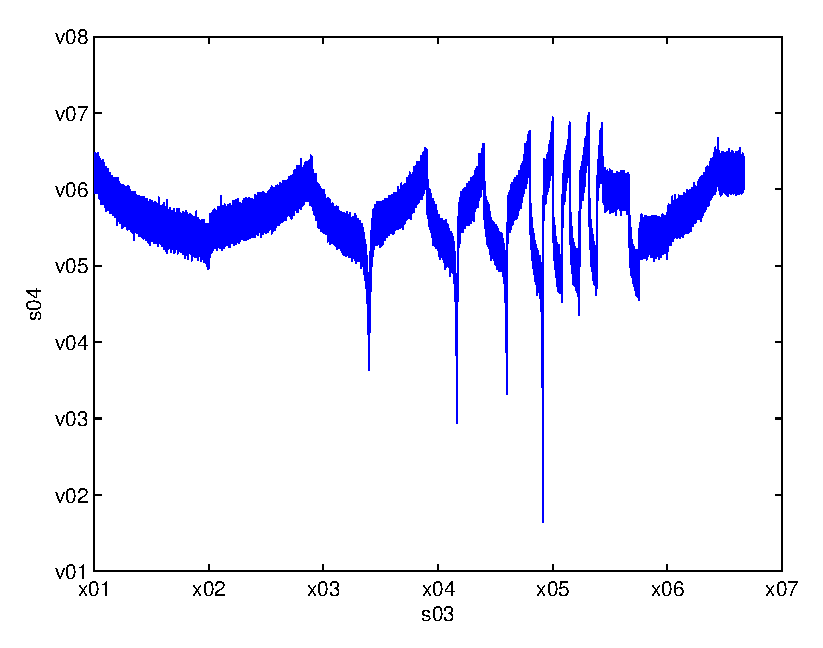
\includegraphics[width=15cm]{meas.eps}%
%\end{psfrags}%
%
% End meas.tex
\end{document}
% See http://www.mathworks.de/matlabcentral/fileexchange/loadFile.do?objectId=4638
% for recent versions of laprint.m.
%
% created by:           LaPrint version 3.16 (13.9.2004)
% created on:           28-Mar-2014 11:29:21
% eps bounding box:     15 cm x 11.0893 cm
% comment:              
%
\begin{psfrags}%
\psfragscanon%
%
% text strings:
\psfrag{s03}[t][t]{\color[rgb]{0,0,0}\setlength{\tabcolsep}{0pt}\begin{tabular}{c}Time [hours]\end{tabular}}%
\psfrag{s04}[b][b]{\color[rgb]{0,0,0}\setlength{\tabcolsep}{0pt}\begin{tabular}{c}$V_\text{cell}$ [V]\end{tabular}}%
%
% xticklabels:
\psfrag{x01}[t][t]{0}%
\psfrag{x02}[t][t]{5}%
\psfrag{x03}[t][t]{10}%
\psfrag{x04}[t][t]{15}%
\psfrag{x05}[t][t]{20}%
\psfrag{x06}[t][t]{25}%
\psfrag{x07}[t][t]{30}%
%
% yticklabels:
\psfrag{v01}[r][r]{1.5}%
\psfrag{v02}[r][r]{2}%
\psfrag{v03}[r][r]{2.5}%
\psfrag{v04}[r][r]{3}%
\psfrag{v05}[r][r]{3.5}%
\psfrag{v06}[r][r]{4}%
\psfrag{v07}[r][r]{4.5}%
\psfrag{v08}[r][r]{5}%
%
% Figure:
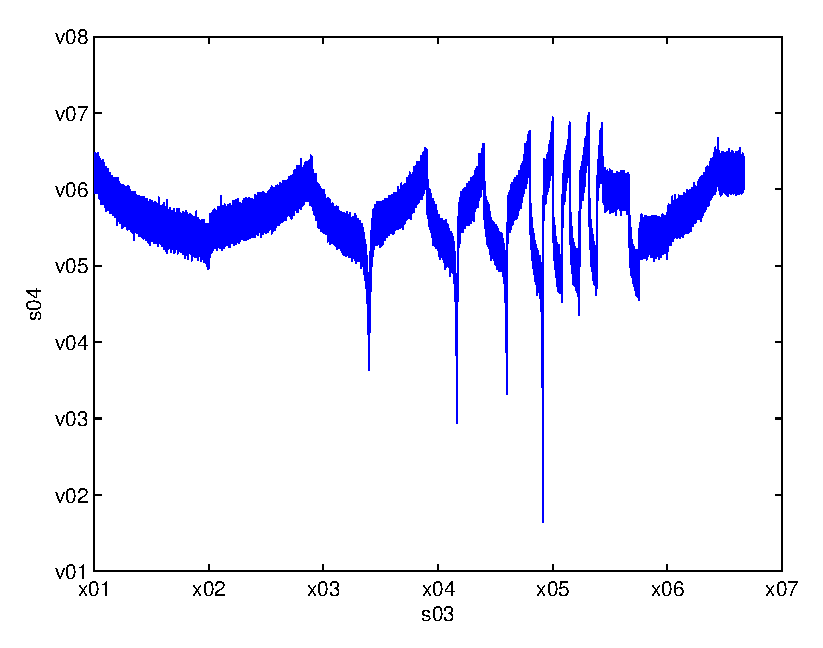
\includegraphics[width=15cm]{meas.eps}%
\end{psfrags}%
%
% End meas.tex
